\label{sec:conclusions}
\par This document has presented a measurement of $\nu_e$ events in the Booster Neutrino Beamline with the MicroBooNE experiment. The analysis leverages sophisticated reconstruction tools which take advantage of scintillation light and detailed calorimetric and spatial information from MicroBooNE's TPC in order to produce a kinematically agnostic measurement of electron neutrinos with any number of final-state protons and no final state pions. The analysis, while aiming to perform a robust measurement across a broad energy range, tailors many of its selection and analysis-level choices to be sensitive to low-energy electron neutrinos, where the complex event topology and high rate of $\nu_{\mu}$ CC and NC backgrounds make the analysis challenging. At the same time, the focus on the sub-GeV energy region allows for analysis sensitivity to anomalies similar to that observed by the MiniBooNE experiment. The analysis reaches a median sensitivity for discovery of a MiniBooNE-like $\nu_e$ signal of $2.3\sigma$ with full statistical, flux, genie, and detector systematics, after the $\nu_{\mu}$ constraint on a dataset of 6.95e20 POT from runs 1,2, and 3. The sensitivity of the analysis is summarized in figure~\ref{fig:sensitivity_bdt_loose_const:conclusions} and table~\ref{tab:sensitivity}.

\begin{figure}[H]
    \begin{center}
    \begin{subfigure}{0.55\textwidth}
    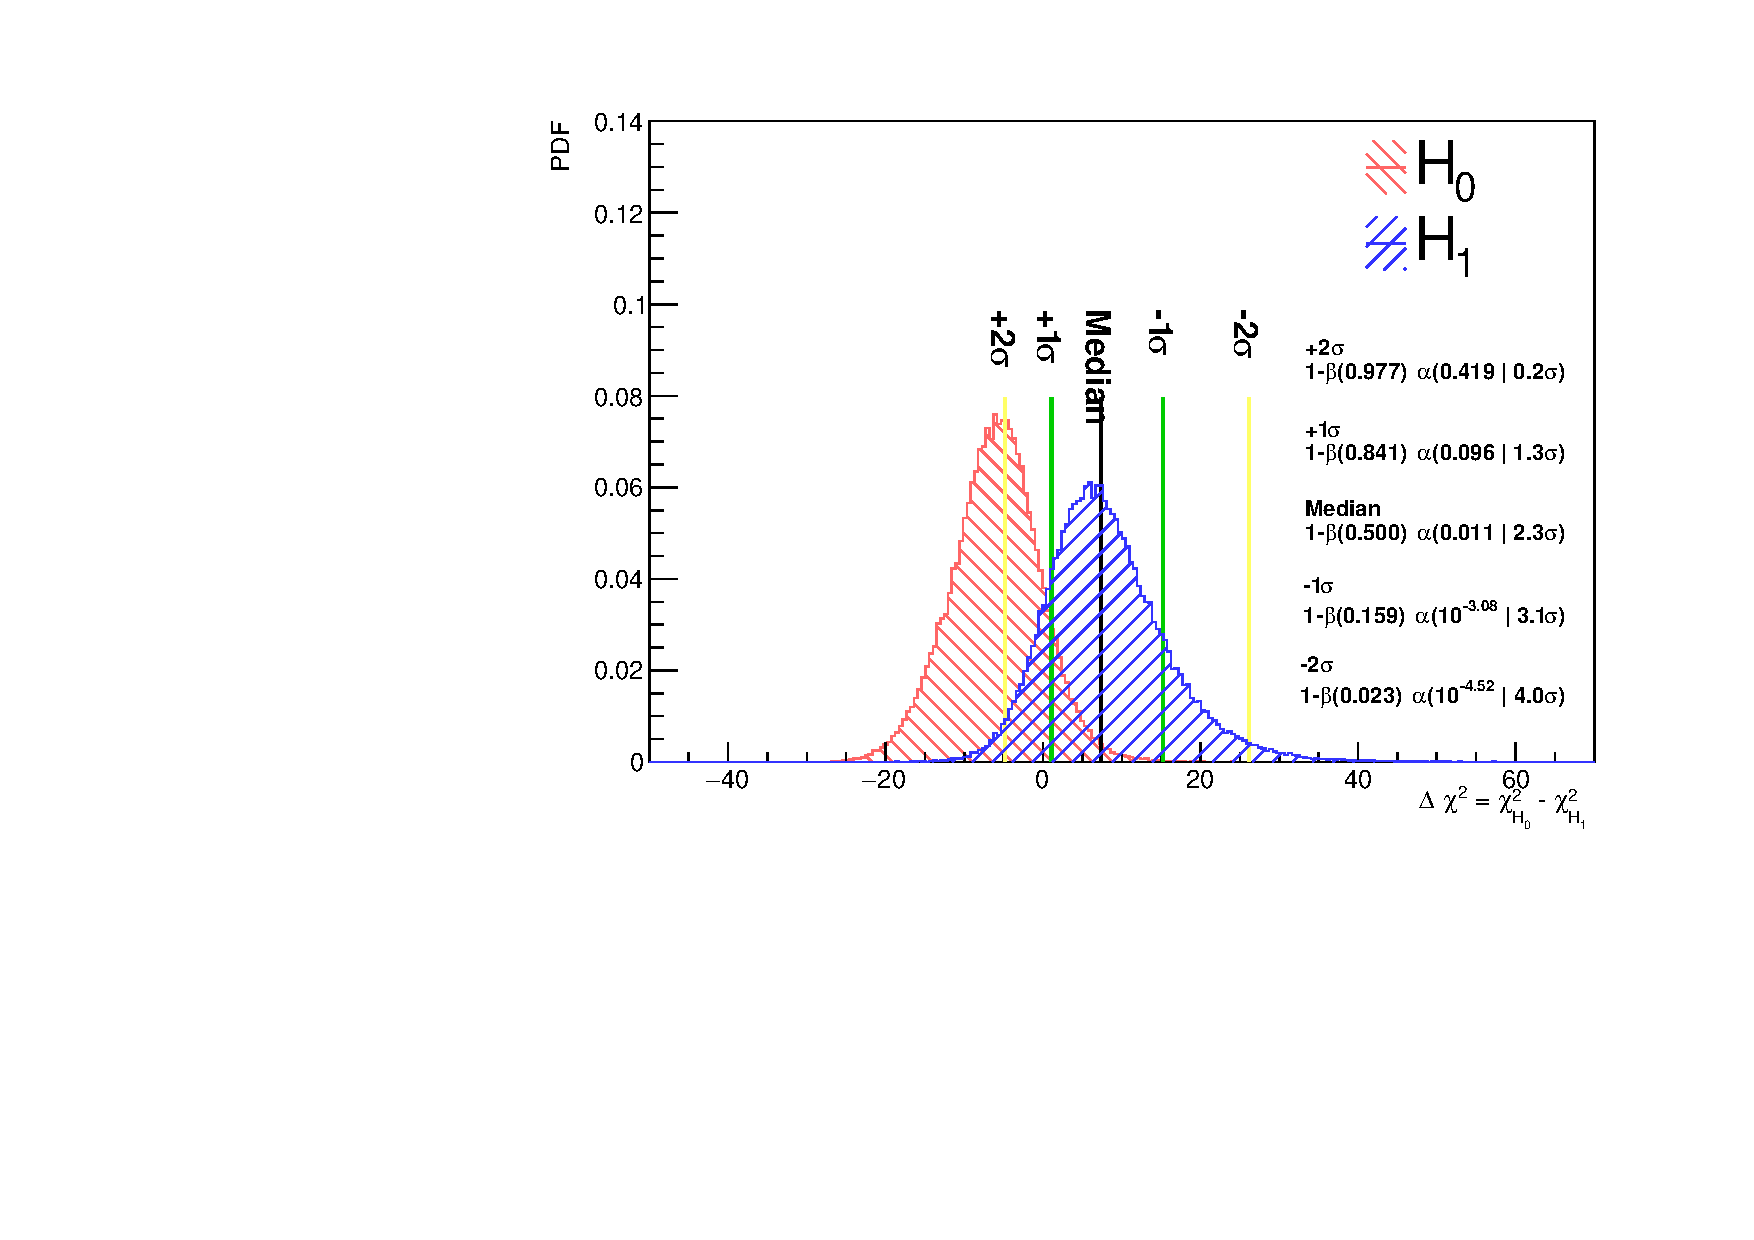
\includegraphics[width=1.00\textwidth]{Sensitivity/sensitivity-run123/SBNfit_Cls_nue_1e0p_numu_reco_e_H1_mc_collab_syst_detsysCNP_Chi.pdf}
    %\caption{Loose BDT selection}
    \end{subfigure}
    \caption{\label{fig:sensitivity_bdt_loose_const:conclusions}Final discovery sensitivity to the LEE unfolded signal of the \npsel selection with the constrained systematics.}
    \end{center}
\end{figure}

\begin{table}[H]
\centering
\setlength{\tabcolsep}{10pt}
\renewcommand{\arraystretch}{1.25}
 \begin{tabular}{| c | c | c | m{2.3 cm} | c | c | c |} 
 \hline
 POT & LEE events & \nue events & scenario & stat. $\sigma$  & stat+syst. $\sigma$ & constrained $\sigma$ \\
 \hline
\multirow{2}{*}{$6.95E20$} &  \multirow{2}{*}{14.97} & \multirow{2}{*}{74.97} & ruling out SM if LEE is true & $2.5$ & $1.9$ & $2.3$ \\
 &  &  & ruling out LEE if SM is true & $2.2$ & $1.9$ & $2.2$ \\
\multirow{2}{*}{$12.5E20$} & \multirow{2}{*}{26.91} & \multirow{2}{*}{134.85} & ruling out SM if LEE is true & $3.3$ & $2.3$ & $3.0$ \\
 &  &  & ruling out LEE if SM is true &$3.0$ & $2.5$ & $2.9$ \\
 \hline
 \end{tabular}
 \caption{\label{tab:sensitivity}Expected sensitivity for run 1-3 data and the run 1-5 data. Event counts are scaled to $6.95E20$ POT and 12.5E20 and include both \npsel and \zpsel LEE signal events.}
\end{table}


\begin{comment}
\begin{table}[H]
\centering
\setlength{\tabcolsep}{10pt}
\renewcommand{\arraystretch}{1.25}
 \begin{tabular}{| c | c | c | c | c | c |} 
 \hline
 channel & LEE events & \nue events & stat. $\sigma$  & stat+syst. $\sigma$ & constrained $\sigma$ \\
 \hline
box-cut \npsel & 10.6 & 51.6 & $2.7$ & $2.3$ & $2.5$ \\
BDT-based \npsel & 14.1 & 74.7 & $2.8$ & $2.3$ & $2.6$ \\
 \hline
 \end{tabular}
 \caption{\label{tab:sensitivity}Expected sensitivity for the Box-Cut and BDT selections of the analysis. Event counts are scaled to $10.1E20$ POT.}
\end{table}
\end{comment}

\par The analysis, as designed and presented, has demonstrated to be robust against detector mis-modeling and time-dependence in MicroBooNE's dataset. The review of this work by the entire MicroBooNE collaboration, if successful, should result in a box-opening of the $6.96e20$ POT collected through Runs 1, 2, and 3. After the processing of data from Runs 4 and 5, and the implementation of specific time-dependent calibrations for such datasets, the analysis will be ready to be processed over the full MicroBooNE dataset.

